\documentclass[journal,12pt,twocolumn]{IEEEtran}
\usepackage{setspace}
\usepackage{gensymb}
\singlespacing
\usepackage[cmex10]{amsmath}
\usepackage{amsthm}
\usepackage{mathrsfs}
\usepackage{txfonts}
\usepackage{stfloats}
\usepackage{bm}
\usepackage{cite}
\usepackage{cases}
\usepackage{subfig}
\usepackage{longtable}
\usepackage{multirow}
\usepackage{enumitem}
\usepackage{mathtools}
\usepackage{steinmetz}
\usepackage{tikz}
\usepackage{circuitikz}
\usepackage{verbatim}
\usepackage{tfrupee}
\usepackage[breaklinks=true]{hyperref}
\usepackage{tkz-euclide}

\usetikzlibrary{calc,math}
\usepackage{listings}
    \usepackage{color}                                            %%
    \usepackage{array}                                            %%
    \usepackage{longtable}                                        %%
    \usepackage{calc}                                             %%
    \usepackage{multirow}                                         %%
    \usepackage{hhline}                                           %%
    \usepackage{ifthen}                                           %%

    \usepackage{lscape}     
\usepackage{multicol}
\usepackage{chngcntr}

\DeclareMathOperator*{\Res}{Res}
\renewcommand\thesection{\arabic{section}}
\renewcommand\thesubsection{\thesection.\arabic{subsection}}
\renewcommand\thesubsubsection{\thesubsection.\arabic{subsubsection}}

\renewcommand\thesectiondis{\arabic{section}}
\renewcommand\thesubsectiondis{\thesectiondis.\arabic{subsection}}
\renewcommand\thesubsubsectiondis{\thesubsectiondis.\arabic{subsubsection}}

\hyphenation{op-tical net-works semi-conduc-tor}
\def\inputGnumericTable{}                                 %%

\lstset{
frame=single, 
breaklines=true,
columns=fullflexible
}

\begin{document}

\newtheorem{theorem}{Theorem}[section]
\newtheorem{problem}{Problem}
\newtheorem{proposition}{Proposition}[section]
\newtheorem{lemma}{Lemma}[section]
\newtheorem{corollary}[theorem]{Corollary}
\newtheorem{example}{Example}[section]
\newtheorem{definition}[problem]{Definition}
\newcommand{\BEQA}{\begin{eqnarray}}
\newcommand{\EEQA}{\end{eqnarray}}
\newcommand{\define}{\stackrel{\triangle}{=}}
\bibliographystyle{IEEEtran}

\providecommand{\mbf}{\mathbf}
\providecommand{\pr}[1]{\ensuremath{\Pr\left(#1\right)}}
\providecommand{\qfunc}[1]{\ensuremath{Q\left(#1\right)}}
\providecommand{\sbrak}[1]{\ensuremath{{}\left[#1\right]}}
\providecommand{\lsbrak}[1]{\ensuremath{{}\left[#1\right.}}
\providecommand{\rsbrak}[1]{\ensuremath{{}\left.#1\right]}}
\providecommand{\brak}[1]{\ensuremath{\left(#1\right)}}
\providecommand{\lbrak}[1]{\ensuremath{\left(#1\right.}}
\providecommand{\rbrak}[1]{\ensuremath{\left.#1\right)}}
\providecommand{\cbrak}[1]{\ensuremath{\left\{#1\right\}}}
\providecommand{\lcbrak}[1]{\ensuremath{\left\{#1\right.}}
\providecommand{\rcbrak}[1]{\ensuremath{\left.#1\right\}}}
\theoremstyle{remark}
\newtheorem{rem}{Remark}
\newcommand{\sgn}{\mathop{\mathrm{sgn}}}
\providecommand{\abs}[1]{\left\vert#1\right\vert}
\providecommand{\res}[1]{\Res\displaylimits_{#1}} 
\providecommand{\norm}[1]{\left\lVert#1\right\rVert}

\providecommand{\mtx}[1]{\mathbf{#1}}
\providecommand{\mean}[1]{E\left[ #1 \right]}
\providecommand{\fourier}{\overset{\mathcal{F}}{ \rightleftharpoons}}

\providecommand{\system}{\overset{\mathcal{H}}{ \longleftrightarrow}}
\newcommand{\solution}{\noindent \textbf{Solution: }}
\newcommand{\cosec}{\,\text{cosec}\,}
\providecommand{\dec}[2]{\ensuremath{\overset{#1}{\underset{#2}{\gtrless}}}}
\newcommand{\myvec}[1]{\ensuremath{\begin{pmatrix}#1\end{pmatrix}}}
\newcommand{\mydet}[1]{\ensuremath{\begin{vmatrix}#1\end{vmatrix}}}
\numberwithin{equation}{subsection}

\makeatletter
\@addtoreset{figure}{problem}
\makeatother
\let\StandardTheFigure\thefigure
\let\vec\mathbf

\renewcommand{\thefigure}{\theproblem}

\def\putbox#1#2#3{\makebox[0in][l]{\makebox[#1][l]{}\raisebox{\baselineskip}[0in][0in]{\raisebox{#2}[0in][0in]{#3}}}}
     \def\rightbox#1{\makebox[0in][r]{#1}}
     \def\centbox#1{\makebox[0in]{#1}}
     \def\topbox#1{\raisebox{-\baselineskip}[0in][0in]{#1}}
     \def\midbox#1{\raisebox{-0.5\baselineskip}[0in][0in]{#1}}
\vspace{3cm}
\title{Assignnment-2}
\author{Vipul Kumar Malik \\ AI20MTECH14006}

\date{\today}

\maketitle
\newpage
\bigskip
\renewcommand{\thefigure}{\theenumi}
\renewcommand{\thetable}{\theenumi}

\begin{abstract}
This document explain the concept of finding the shortest distance between lines.
\end{abstract}
Download all python codes from 
\begin{lstlisting}
https://github.com/vipulmalik8569/MT-EE5609
\end{lstlisting}
and latex-tikz codes from 
\begin{lstlisting}
https://github.com/vipulmalik8569/MT-EE5609
\end{lstlisting}

\section{\textbf{Problem}}

Find the shortest distance between the lines :
\begin{align}
L_1 :\vec{x} &= \myvec{ 1-t \\ t-2 \\ 3-2t } = \myvec{1\\-2\\3}+ t\myvec{-1\\1\\-2}\\
L_2 :\vec{x} &= \myvec{ s+1 \\ 2s-1 \\ -2s-1 } = \myvec{1\\-1\\-1}+ s\myvec{1\\2\\-2} 
\end{align}

\section{\textbf{Solution}}
We have,
\begin{align}
    L_1 : \vec{x}= \vec{a_1} + t \vec{b_1}\label{eq:1}\\
    L_2 : \vec{x}= \vec{a_2} + s \vec{b_2}\label{eq:2}
\end{align}

where, $\vec{a_i}$, $\vec{b_i}$ are positional and slope vectors of line $L_i$ respectively.\\

As $\vec{b_1}\neq \lambda \vec{b_2}$, lines $L_1$ and $L_2$ are not parallel to each other.\\

Now, let us assume that $L_1$ and $L_2$ are intersecting at a point. Therefore,
\begin{align}
{\myvec{1\\-2\\3}+ t\myvec{-1\\1\\-2}&=\myvec{1\\-1\\-1}+ s\myvec{1\\2\\-2}}\\
s\myvec{-1\\-2\\2} + t\myvec{-1\\1\\-2}&=\myvec{0\\1\\-4}\\
\myvec{-1&-1\\-2&1\\2&-2} \myvec{s\\t}&=\myvec{0\\1\\-4}
\end{align}
Using Gaussian elimination method:
\begin{align}
 E=E_{32}E_{31}E_{21}&=\myvec{1&0&0 \\ -2&1&0 \\\frac{-1}{2}&1&\frac{3}{4}}\\
 E\myvec{-1&-1&:&0\\-2&1&:&1\\2&-2&:&-4}&=\myvec{-1&-1&:&0\\0&3&:&1\\0&0&:&-2}\label{eq:7}
\end{align}\\

From \eqref{eq:7} it is clear that the system of linear equations are inconsistent. Therefore $L_1$ and $L_2$ are not intersecting at any point. 

Hence our assumption was wrong, $L_1$, $L_2$ are \textbf{skew lines}.

Let $d$ be the shortest distance  between $L_1$, $L_2$ and $\vec{p_1}$, $\vec{p_2}$ be the positional vectors of its end points.

For $d$ to be the shortest, we know that,
\begin{align}
\vec{b_1}^T(\vec{p_2}-\vec{p_1})=0\\
\vec{b_2}^T(\vec{p_2}-\vec{p_1})=0\\
\vec{b_1}^T\left((\vec{a_2}-\vec{a_1})+\myvec{\vec{b_2}&\vec{b_1}}\myvec{s\\-t}\right)=0\label{eq:10}\\
\vec{b_2}^T\left((\vec{a_2}-\vec{a_1})+\myvec{\vec{b_2}&\vec{b_1}}\myvec{s\\-t}\right)=0\label{eq:11}\\
\vec{B}= \myvec{\vec{b_2}&\vec{b_1}}, \vec{B^T}= \myvec{\vec{b_2}^T\\\vec{b_1}^T}\label{eq:12}
\end{align}
By combining equation \eqref{eq:10} and \eqref{eq:11} and writing in terms of $\vec{B}$ and $\vec{B}^T$ using \eqref{eq:12} we get:
\begin{align}
\vec{B}^T\vec{B}\myvec{s\\-t}&=\vec{B}^T(\vec{a_1}-\vec{a_2})\label{eq:13}
\end{align}
By putting the values of $\vec{a_1}, \vec{a_2}, \vec{b_1}$ and $\vec{b_2}$ in equation \eqref{eq:13} we get:
\begin{align}
\myvec{5&6\\9&5}\myvec{s\\-t}&=\myvec{-9\\-10}\label{eq:14}\label{eq:14}
\end{align}
Solving equation \eqref{eq:14} we get:
\begin{align}
    s=\frac{-15}{29}, t=\frac{31}{29}
\end{align}

By putting the values of $t$ and $s$ in equation \eqref{eq:1} and \eqref{eq:2} respectively we get:
\begin{align}
    \vec{p_1}=\myvec{\frac{-17}{250}\\[0.2cm]\frac{-93}{100}\\[0.2cm]\frac{43}{50}},\vec{p_2}=\myvec{\frac{12}{25}\\[0.2cm]-2\\[0.2cm]\frac{17}{500}}
\end{align}
Hence the shortest distance $d$ between the two skew lines is :
\begin{align}
d=\norm{\vec{p_2}-\vec{p_1}}=1.4855
\end{align}
\begin{figure}[h]
\centering
    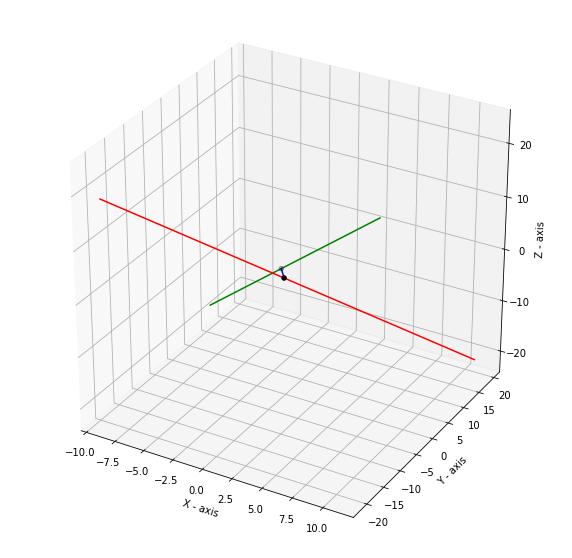
\includegraphics[width=\columnwidth]{assignment2.png}
    \caption{3-D plot for the skew lines and the shortest distance between them.}
    \label{skew_lines}
\end{figure}
\end{document}

